\documentclass[11pt]{article}
\usepackage[margin=1in]{geometry}
\usepackage{amsmath,amssymb,amsthm,mathtools}
\usepackage{graphicx}
\usepackage{hyperref}
\usepackage{xcolor}

\newtheorem{theorem}{Theorem}
\newtheorem{lemma}[theorem]{Lemma}
\newcommand{\R}{\mathbb R}
\newcommand{\N}{\mathbb N}
\newcommand{\qG}{\mathrm{q}\mathcal G^*}

\title{A Closed Pointed Cone Outside $\qG$\
for Which the Bounded-Base Equivalence Holds}
\author{Automatic mathematics run \texttt{fa\_banach\_001}}
\date{9 August 2026}

\begin{document}
\setlength{\emergencystretch}{3em}
\maketitle

\begin{center}
\fbox{\parbox{0.91\textwidth}{
\textbf{Status.} Candidate counterexample, likely valid, for human review.
It gives a full negative answer to Problem~1 of
Garc\'ia-Casta\~no--Melguizo Padial, including under the natural restriction
to closed pointed cones in Banach spaces.
}}
\end{center}

\section{Source problem}

For a cone $C$ in a normed space $X$, let
\[
 C^*=\{f\in X^*:f(c)\geq0\text{ for every }c\in C\}.
\]
The family $\qG$ consists of the cones whose dual cone is
quasi-generating, that is,
\[
 \overline{C^*-C^*}^{\|\cdot\|}=X^*.
\]
Garc\'ia-Casta\~no and Melguizo Padial prove that if $C\in\qG$, then
\[
 \left[
 0\notin\overline{C\setminus\epsilon B_X}^{\,\mathrm{weak}}
 \quad\text{for every }\epsilon\in(0,1)
 \right]
 \quad\Longleftrightarrow\quad
 [C\text{ has a bounded base}].                         \tag{1}
\]
Their Problem~1 asks whether $\qG$ is maximal among families of cones for
which (1) holds \cite{source}.  Since their motivation explicitly notes that
closed cones need not belong to $\qG$, it is useful to answer the question
without exploiting a nonclosed or nonpointed cone.

The complete source page, including the definition of a base, Corollary~1,
and Problem~1, follows.

\clearpage
\begin{center}
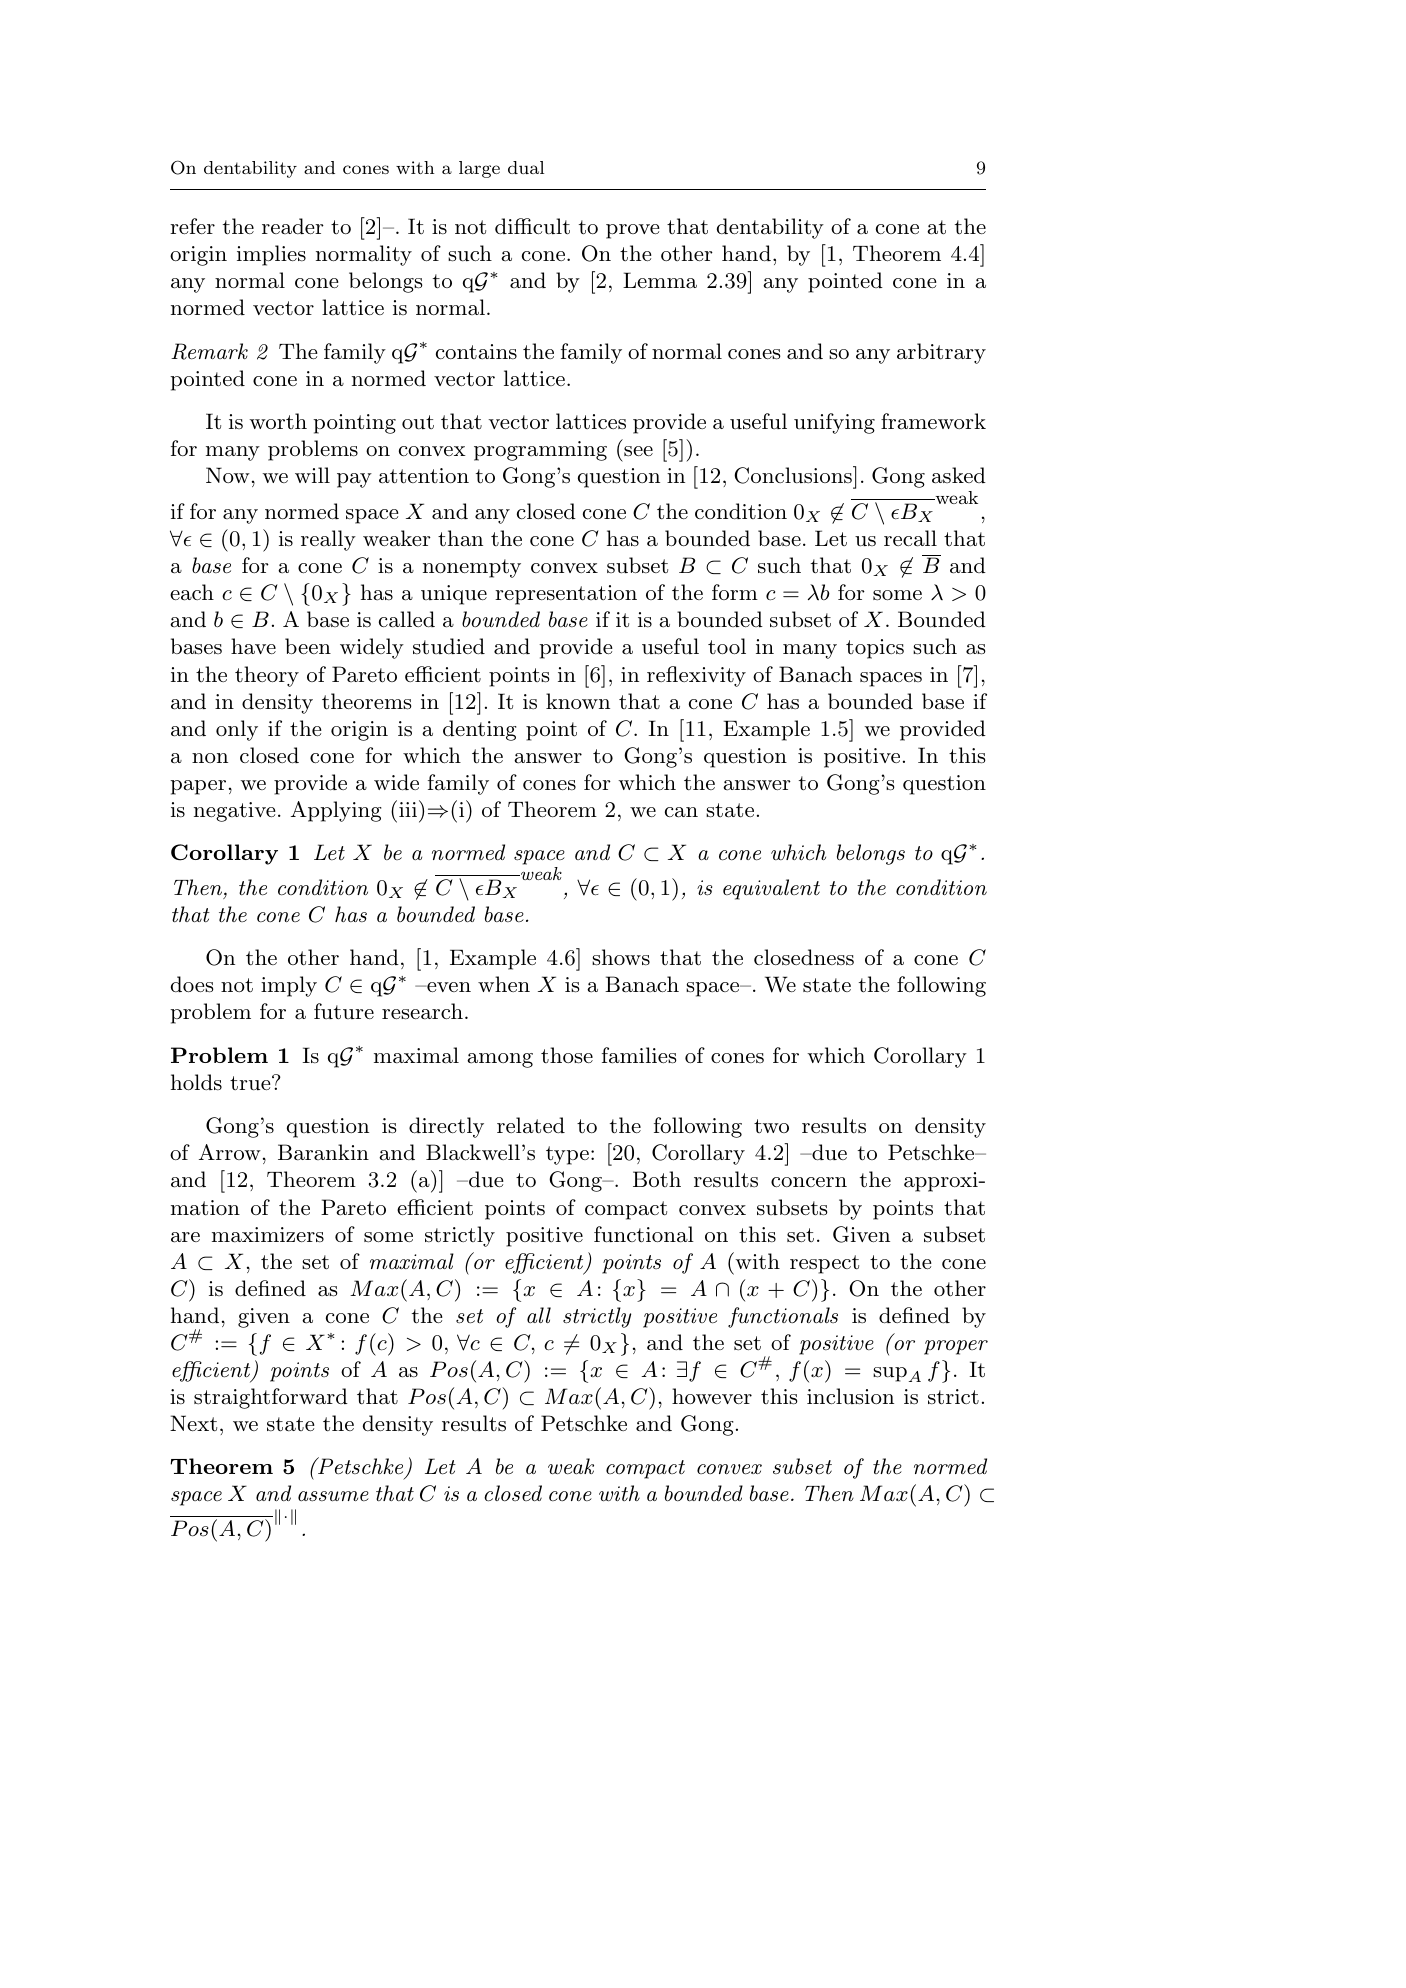
\includegraphics[width=0.96\textwidth]{figures/source_problem_page9.png}
\end{center}

\section{Proof intuition}

An epigraph cone converts the geometry of an auxiliary norm into order
geometry.  We choose a continuous but much weaker norm $p$ on $c_0$ with two
special sequences.  First, the usual unit vectors have ambient norm one but
$p$-norm tending to zero; their lifts to the boundary of the epigraph are
therefore weakly null points of norm one.  This simultaneously destroys the
weak separation condition and every bounded base.  Second, the initial-block
vectors $e_1+\cdots+e_N$ have $p$-norm tending to zero.  Positivity of a dual
functional on both signs of these boundary vectors then forces the sum of its
$\ell^1$ coordinates to vanish.  Thus the entire dual cone spans only a proper
hyperplane.  The epigraph remains closed and pointed because $p$ is a genuine
continuous norm.

\section{Construction and proof}

Work over the real field.  Put
\[
 E=c_0(\N),
 \qquad
 X=E\oplus_\infty\R,
 \qquad
 \|(x,t)\|=\max\{\|x\|_\infty,|t|\}.
\]
Define, for $x=(x_k)_{k\geq1}\in c_0$,
\[
 p(x):=\sup_{k\geq1}2^{-k}|x_k-x_{k+1}|.                \tag{2}
\]
The function $p$ is a norm on $c_0$: if all successive differences vanish,
then $x$ is constant, hence $x=0$ because $x\in c_0$.  Moreover
$p(x)\leq\|x\|_\infty$, so $p$ is continuous for the usual norm.

Consider its epigraph cone
\[
 C:=\{(x,t)\in X:t\geq p(x)\}.                           \tag{3}
\]

\begin{theorem}\label{thm:main}
The cone $C$ in \emph{(3)} is closed and pointed, but $C\notin\qG$.
Nevertheless, the two assertions in \emph{(1)} are both false for $C$.
Consequently $\qG$ is not maximal among families of cones for which
\emph{(1)} holds.  This remains true if the ambient class is restricted to
closed pointed cones in Banach spaces.
\end{theorem}

\begin{proof}
Since $p$ is continuous and convex, its epigraph $C$ is a closed convex cone.
If both $(x,t)$ and $(-x,-t)$ belong to $C$, then
\[
 t\geq p(x)
 \quad\text{and}\quad
 -t\geq p(-x)=p(x).
\]
Thus $p(x)=0$ and $t=0$, whence $x=0$.  Therefore $C$ is pointed.

We next show that its dual cone is not quasi-generating.  Identify
$X^*=\ell^1\oplus_1\R$ and write its elements as $(f,a)$, acting by
\[
 \langle(f,a),(x,t)\rangle=\sum_{k\geq1}f_kx_k+at.
\]
Positivity on $(0,t)$ for all $t\geq0$ forces $a\geq0$.  Positivity on the
boundary points $(x,p(x))$ and $(-x,p(x))$ then gives
\[
 \left|\sum_{k\geq1}f_kx_k\right|\leq a p(x)
 \qquad(x\in c_0).                                      \tag{4}
\]
Conversely, $a\geq0$ and (4) plainly suffice for $(f,a)\in C^*$.

Let $s_N=e_1+\cdots+e_N$.  Then $p(s_N)=2^{-N}$, so (4) yields
\[
 \left|\sum_{k=1}^Nf_k\right|\leq a2^{-N}.
\]
Because $f\in\ell^1$, passage to the limit gives
\[
 \sum_{k\geq1}f_k=0.                                    \tag{5}
\]
Hence
\[
 C^*-C^*\subset
 \left\{(f,a)\in\ell^1\oplus_1\R:
              \sum_{k\geq1}f_k=0\right\}.              \tag{6}
\]
The right-hand side is a proper norm-closed hyperplane of $X^*$.
Thus $C^*-C^*$ is not norm dense and $C\notin\qG$.

It remains to test (1).  For $n\geq2$ let
\[
 u_n=(e_n,p(e_n))\in C.
\]
Here $p(e_n)=2^{-(n-1)}$, so $p(e_n)\to0$.  The canonical unit vectors are
weakly null in $c_0$, and therefore
\[
 u_n\rightharpoonup0\quad\text{in }X,
 \qquad \|u_n\|=1.                                     \tag{7}
\]
For every $\epsilon\in(0,1)$, the entire sequence lies in
$C\setminus\epsilon B_X$.  Equation (7) proves
\[
 0\in\overline{C\setminus\epsilon B_X}^{\,\mathrm{weak}}
 \qquad\text{for every }\epsilon\in(0,1),               \tag{8}
\]
so the left assertion in (1) is false.

For completeness, (7) also directly rules out a bounded base.  Indeed,
suppose $B$ were a bounded base for $C$.  By the definition used in the
source, $B$ is convex and $0\notin\overline B$.  Strong separation gives
$\Phi\in X^*$ and $\alpha>0$ such that
$\Phi(b)\geq\alpha$ for every $b\in B$.  Put
$M=\sup_{b\in B}\|b\|<\infty$.  Every $c\in C\setminus\{0\}$ has the
form $c=\lambda b$, and if $\|c\|\geq\epsilon$ then
$\lambda\geq\epsilon/M$.  Consequently
\[
 \Phi(c)\geq\frac{\alpha\epsilon}{M}
 \qquad(c\in C\setminus\epsilon B_X).                  \tag{9}
\]
The weak neighborhood
$\{x\in X:|\Phi(x)|<\alpha\epsilon/(2M)\}$ of zero is disjoint from the
truncated cone, contradicting (8).  Thus $C$ has no bounded base, so the
right assertion in (1) is false as well.

Both sides of (1) are false, hence their equivalence holds for $C$.
Adjoining this single cone to $\qG$ produces a strictly larger family on
which (1) holds, which proves the maximality claim false.
\end{proof}

\section{Scope}

The example does not merely exploit the fact that the source definition of
a cone allows nonpointed or nonclosed sets.  It is a closed pointed cone in
the Banach space $c_0\oplus_\infty\R$, precisely the setting suggested by the
sentence immediately preceding Problem~1.  The conclusion is the literal
set-theoretic nonmaximality asked there.  It does not propose a maximal
\emph{natural} or structurally defined replacement for $\qG$.

\section{Verification and novelty scope}

Every substantive step is contained in (2)--(9).  In particular, the dual
obstruction is witnessed by the explicit continuous functional
$(f,a)\mapsto\sum_k f_k$ on $X^*$, and the bounded-base obstruction is
witnessed by an explicit weakly null sequence of norm one.

A bounded literature audit was performed on 9 August 2026 after the direct
construction.  The run indexes, exact-phrase and core-keyword web searches,
the current arXiv record, the 2019 journal version, and later papers citing
the source were checked.  No later resolution of Problem~1 or occurrence of
this epigraph-cone example was found.  This supports plausible novelty only;
it does not certify priority.

\begin{thebibliography}{9}
\bibitem{source}
F. Garc\'ia-Casta\~no and M. A. Melguizo Padial,
\emph{On dentability and cones with a large dual},
Rev. R. Acad. Cienc. Exactas F\'is. Nat. Ser. A Mat. RACSAM
\textbf{113} (2019), 2679--2690;
\href{https://doi.org/10.1007/s13398-019-00650-3}{doi:10.1007/s13398-019-00650-3},
also \href{https://arxiv.org/abs/2401.10102}{arXiv:2401.10102}.
\end{thebibliography}

\end{document}
